% simon.dobnik@gu.se

\documentclass[aspectratio=1610]{beamer} % alternative: 169

\usepackage[1610]{gu-slides} % alternative: 16:9

\usepackage{graphicx,hyperref,natbib}
\usepackage[utf8]{inputenc}


\usepackage{amsmath}
\DeclareSymbolFont{matha}{OML}{txmi}{m}{it}% txfonts
\DeclareMathSymbol{\varv}{\mathord}{matha}{118}
\usepackage{subfig}
\newcommand{\squeezeup}{\vspace{-3mm}}
\newcommand{\squeezedown}{\vspace{2.5mm}}
\captionsetup[subfigure]{labelformat=empty}

\usepackage{tikz}
\newcommand\tikznode[3][]%
{\tikz[remember picture,baseline=(#2.base)]
    \node[minimum size=0pt,inner sep=0pt,#1](#2){#3};%
}

\usepackage{xcolor}
\usepackage{arydshln}
\setlength{\dashlinedash}{5pt}
\setlength{\dashlinegap}{4pt}

\newcommand{\rulesep}{\unskip\ \vrule\ }



\title{Examining the Effects of Language-and-Vision Data Augmentation for Generation of Descriptions of Human Faces}

\author{
Nikolai Ilinykh$^{\ast}$ \and Rafal Černiavski$^{\dagger}$ \and Eva Elžbieta Sventickaitė$^{\dagger}$ \\ \and Viktorija Buzaitė$^{\dagger}$ \and Simon Dobnik$^{\ast}$ \\
	\vspace{.2cm}
        \small $^{\ast}$Centre for Linguistic Theory and Studies in Probability (CLASP), \\
        Department of Philosophy, Linguistics and Theory of Science (FLoV), \\
        University of Gothenburg, Sweden \\
	$^{\dagger}$Faculty of Languages, Department of Linguistics and Philology, \\ Uppsala University, Sweden \\
	\vspace{.2cm}
	\texttt{nikolai.ilinykh, simon.dobnik@gu.se}$^{\ast}$ \\
	\texttt{rafal.cerniavski.2286, evaelzbieta.sventickaite.9060, viktorija.buzaite.1828@student.uu.se}$^{\dagger}$ \\
      }

\date{P-VLAM 2022, co-located with LREC 2022}

% 15 mins max, 5 mins for questions

\begin{document}




\frame[plain]{\titlepage}


%\frame[plain]{\frametitle{Outline}\tableofcontents}

\begin{frame}
\frametitle{Why?}

\begin{itemize}

\vspace{.7cm}
\item Building face description systems is beneficial for humans with prosopagnosia.
% The lack of the ability to recognise and describe a human face has underlying social importance for people with neurological conditions.
% Therefore in this study we focused on the task of automatic generation of description of faces since developing such systems is potentially beneficial for humans with specific neurological conditions.
\pause
\item Face recognition and description is central to social interaction and it has an impact on decision-making and inter-personal relations.
% In other words, describing faces has a social impact once we think of the models for automatic description of faces.
% Thus it is important to monitor the quality of automatically generated descriptions of faces.
% Because many descriptions contain subjective opinions (e.g., beautiful, old) and it is important to have a system that does not discriminate humans based on their facial features.
% SD: Swap point 1 and 2?
\pause
\item Face description generation involves subjective language and requires a fine-grained understanding of specific parts of images (in \textcolor{blue}{blue}).
% Mapping these descriptions with visual features is hard
%\item Face description generation requires a fine-grained understanding of the image.
% Image captioning is viewed as the standard multi-modal task and progress on this task has been truly astonishing.
% However, describing human faces is a very different task, which requires deeper understanding of specific parts in the image.
% While standard image captions describe images in general, mentioning all salient objects, descriptions of faces focus a lot on parts and attributes of the specific object (that is, the 'face' objects)

\end{itemize}

\vspace{-.3cm}
%\squeezedown
%An example image (original \& with detected objects):
%\squeezeup
\begin{figure}[htbp]
\centering
\subfloat{
    \frame{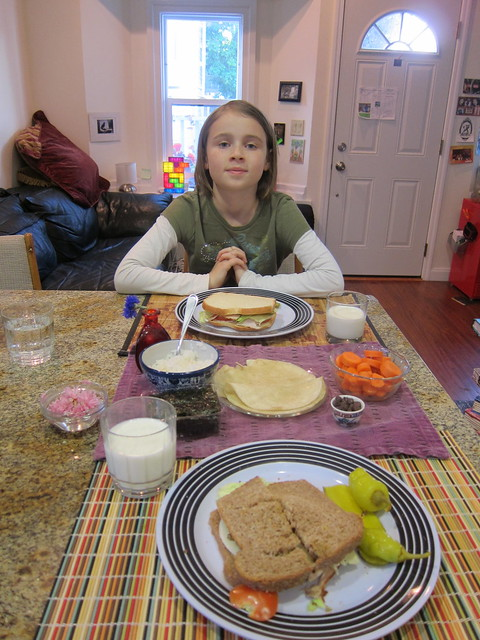
\includegraphics[width=20mm]{cocoexample}}}
  %\qquad
 \subfloat[]{
   \noindent%
    \parbox[b]{.2\textwidth}{%
    	\textbf{COCO:}\\
        A girl is sitting at a table set with sandwiches and milk.
    }%
    }
%\qquad
\subfloat[]{
    {\raisebox{1ex}% select appropriate amount
            { \frame{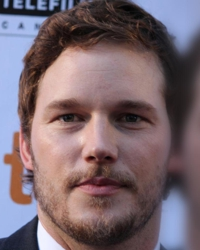
\includegraphics[width=20mm]{9737}}}%
            %\frame{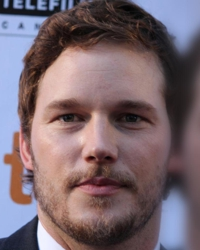
\includegraphics[width=40mm]{9737}}
            }
            }
%\qquad
\subfloat[]{
   \noindent%
    \parbox[b]{.2\textwidth}{%
    	\textbf{CelebA-HQ:}\\
        The person has \textcolor{blue}{big lips, sideburns, goatee, mustache, and brown hair}. He is wearing necktie.
    }%
    }

\label{fig:taskdiff}
\end{figure}
\bigskip
\end{frame}


\begin{frame}
\frametitle{In this study we \ldots}
\begin{itemize}
	\item Examine the fit of a standard image description generation model for face description generation.
	% We take a simple CNN-LSTM model that takes an image of a face as its input and generates description in auto-regressive fashion
	% For training, we use CelebA-HQ dataset.  The dataset contains 30, 000 high-resolution images of human faces of celebrities with 10 natural language descriptions per each image.
	% We aim to examine the extent to which a standard captioning model is useful for face description generation task.
	\item Analyse the impact of different feature representations on face description generation.
	% We perform several experiments in which we modify either visual or linguistic inputs to the model.
	% Our goal is to evaluate the robustness of the model when presented with different feature types.
	\item Evaluate the quality of visual abstractions for facial feature classification.
	% We also test different visual representations for a different task of feature classification.
	% With this, we aim to evaluate the quality of visual abstractions.
        % SD: Test the effects of text augmentation on the quality of descriptions?
\end{itemize}
% Our results show that 
\end{frame}

\begin{frame}
\frametitle{Visual augmentation}
\begin{figure}[htbp]
\centering
\frame{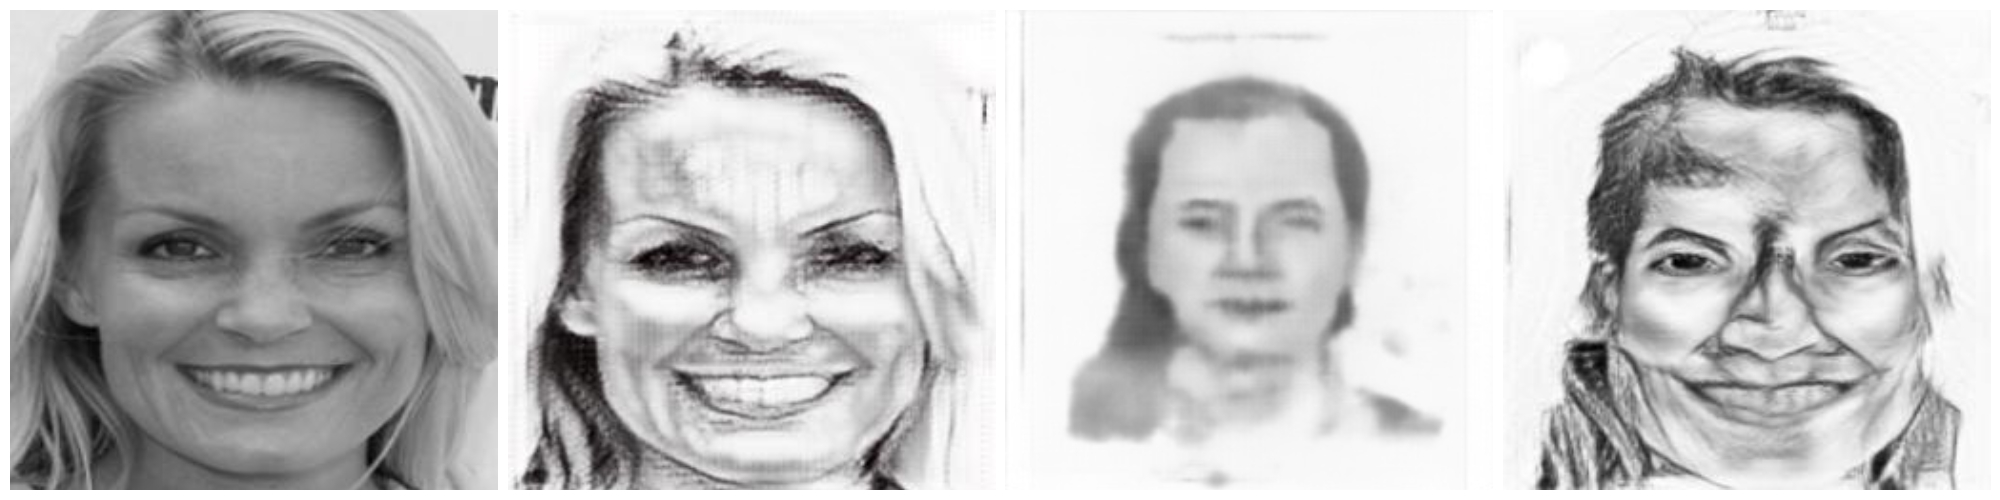
\includegraphics[width=10cm, scale=0.2]{1.jpg}}
\label{fig:generalexample}
\end{figure}
\begin{itemize}
	\item We train a description generation model on different visual abstractions. % (shown above).
	\item From left to right: \textbf{original, composite, sketch, distorted}.
	\item Sketches are generated by applying an auto-encoder on original images.
	\item Composites are generated by a GAN trained for $5$ epochs; distorted images are generated by the same GAN but after $33$ epochs.
	% What do we expect from the model that is provided with different visual abstractions? A better or comparable performance with the original images.
	% Why? Because abstractions bring to the fore more distilled representations (general facial features on sketches are much more pronounced, e.g., shapes and sizes of parts of the faces)
	% At the same time, abstract sketches look much more similar to each other, while original images are much more varied in terms of individual features. Therefore, at the same time we reduce visual representations to only such which are potentially essential for face description generation.
\end{itemize}
\end{frame}


\begin{frame}
\frametitle{Linguistic augmentation}

\vspace{-.3cm}
%\squeezedown
%An example image (original \& with detected objects):
%\squeezeup
\begin{figure}[htbp]
\centering
\subfloat{
    \frame{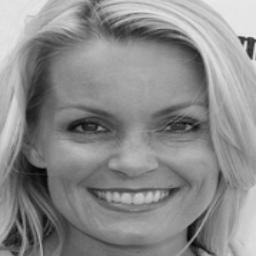
\includegraphics[width=30mm]{image}}}
  \qquad
 \subfloat[]{
   \noindent%
    \parbox[b]{.3\textwidth}{%
    	\textbf{Original:}\\
       This person is \textcolor{red}{attractive}, and  \textcolor{red}{young} and  \textcolor{red}{has bags} under eyes,  \textcolor{red}{wavy} hair,  \textcolor{red}{arched} eyebrows, and mouth  \textcolor{red}{slightly open}.
    }%
    }
%\qquad
\hspace{.5cm}
\subfloat[]{
   \noindent%
    \parbox[b]{.3\textwidth}{%
    	\textbf{Augmented:}\\
        This person is  \textcolor{red}{not unattractive}, and  \textcolor{red}{not old} and  \textcolor{red}{doesn't have flat} under eyes,  \textcolor{red}{straight} hair,  \textcolor{red}{straight} eyebrows, and mouth  \textcolor{red}{completely closed}.
    }%
    }

\label{fig:lingaug}
\end{figure}
\vspace{-.5cm}
\begin{itemize}

	\item We also train a model with original images but different/augmented descriptions.
	\item We replace verbs, adjectives and adverbs with their antonyms and negate them.
	\item The idea is to produce a description that is semantically close to the original text but different in terms of their form. %(augmentation on the textual side).
	\item We also augment original dataset with a subset of the Flickr8k dataset, bringing semantic knowledge from a different multi-modal domain.
	% We went with this method after trying multiple automatic augmentation methods that use different embeddings (either glove, w2v or contextual transformer embeddings) to find either synonyms or antonyms and replace words in text with them. We also tried to search wordnet for either synonyms or antonyms. On the text side, we were either substituting words or inserting them. More details and evaluation of the results from these methods are available in the paper. In the end we decided to go with our own manual method that seemed to produce the least number of wrong substitutions.
	% with flickr8k we aim to 

\end{itemize}
\end{frame}


\begin{frame}
\frametitle{Generation: training details}
\begin{itemize}

	\item A simple CNN-LSTM with attention.
	\item The best model is chosen based on BLEU on the validation set after $20$ epochs.
	\item Decoding: greedy.
	\pause
	\item The models we train:
		\begin{itemize}
			\item \textcolor{red}{Visual augmentation}:
			\item \textbf{Baseline}: original captions and images
			\item \textbf{GAN:Composite}: original captions and composite images (after 5 epochs)
			\item \textbf{GAN:Distorted}: original captions and composite images (after 33 epochs)
			\item \textbf{Face-2-Sketch}: original captions and sketches  
			\item[] ----------
			\item \textcolor{red}{Linguistic augmentation}:
			\item \textbf{Aug-Anton 3:2}: original images with 3 original and 2 augmented captions each
			\item \textbf{Aug:Anton 5}: original images with 5 augmented captions each
			\item \textbf{Aug-Caption}: original dataset plus a subset of Flickr8k
		\end{itemize}

\end{itemize}
\end{frame}


% We evaluate models in terms of three text generation metrics: METEOR, BLEU-1 and ROUGE
% All models were trained with different feature modifications on either visual or linguistic side, but each of them was evaluated on three types of visual representations: original images (first column), composites (second column) and distorted (third column).
% I am going to colour relevant parts in red and discuss them one after another.

% First, we will look at the differences between models in the experiment with visual augmentations
% The first important result is that the model that is trained with sketches performa in par with the baseline when evaluated on original images
% It has the same performance in terms of METEOR, and it is second (in terms of performance) model (that was trained on original images) in terms of BLEU-1 and ROUGE
% It indicates that either (i) the baseline is bad because it performs close to the sketch model, so the baseline cannot fully use original visual representations because they are either of bad quality or the model is bad (ii) or the model is actually able to sufficiently learn from sketches of faces.

\begin{frame}
\frametitle{Results}

\begin{table}[htbp]
\small
\centering
\resizebox{.45\textwidth}{!}{
\begin{tabular}{|l|rrr|}
\hline
\textbf{METEOR} & \textbf{1. img} & \textbf{2. cmp} & \textbf{3. dst} \\ 
\hline
A. Baseline & \textcolor{red}{72.87}
                                                          & 60.27                                                              & 60.35                                                               \\
B. GAN:Composite        & 59.47                                                             & 72.76                                                           & 66.95                                                               \\
C. Face-2-Sketch       & \textcolor{red}{72.87}                                                          & 61.86                                                              & 61.36                                                               \\
D. GAN:Distorted         & 57.17                                                             & 64.22                                                              & 70.93                                                          \\
\hdashline
E. Aug-Caption             & 69.98                                                             & 39.06                                                              & 46.03                                                               \\
F. Aug-Anton 3:2 & 72.51                                                         & 62.34                                                         & 61.29                                                         \\
G. Aug-Anton 5   & 41.02                                                             & 32.71                                                              & 33.35                                                               \\
\hline
\hline
\textbf{BLEU-1} & \textbf{1. img} & \textbf{2. cmp} & \textbf{3. dst} \\ 
\hline
A. Baseline          & 48.12                                                  & 30.41                                                     & 29.18                                                      \\
B. GAN:Composite        & 26.84                                                    & 43.76                                               & 33.71                                                      \\
C. Face-2-Sketch       & \textcolor{red}{39.91}                                                 & 24.22                                                     & 25.39                                                      \\
D. GAN:Distorted         & 27.75                                                    & 36.29                                                     & 43.69
\\
\hdashline
E. Aug-Caption             & 49.71                                                  & 12.94                                                     & 17.79                                                      \\
F. Aug-Anton 3:2 & 39.09                                                    & 30.65                                                & 32.41                                                 \\
G. Aug-Anton 5   & 13.84                                                    & 7.10                                                      & 8.71                                                       \\
\hline
\hline
\textbf{ROUGE} & \textbf{1. img} & \textbf{2. cmp} & \textbf{3. dst} \\ 
\hline
A. Baseline          & 64.36                                                  & 53.13                                                     & 54.41                                                      \\
B. GAN:Composite        & 54.36                                                    & 62.07                                                & 57.67                                                      \\
C. Face-2-Sketch       & \textcolor{red}{59.58}                                                & 50.11                                                     & 51.19                                                      \\
D. GAN:Distorted         & 53.27                                                    & 62.07                                                     & 62.65                                                   \\
\hdashline
E. Aug-Caption             & 65.81                                                & 44.41                                                     & 48.03                                                      \\
F. Aug-Anton 3:2 & 59.46                                                    & 54.31                                                 & 54.08                                                     \\
G. Aug-Anton 5  & 42.33                                                    & 35.52                                                     & 35.76                                                      \\
\hline
\end{tabular}
}
\label{fig:results}
\end{table}
\end{frame}


% Next, as expected, across all metrics all models performed the best when evaluate on the same type of features that they were trained on.
% Interestingly, performance of two GAN-based models was identical in terms of ROUGE when evaluate on composites. It might indicate that the captioning model cannot differentiate between composites and distorted images, although they look drastically different.

\begin{frame}
\frametitle{Results}

\begin{table}[htbp]
\small
\centering
\resizebox{.45\textwidth}{!}{
\begin{tabular}{|l|rrr|}
\hline
\textbf{METEOR} & \textbf{1. img} & \textbf{2. cmp} & \textbf{3. dst} \\ 
\hline
A. Baseline &  \textcolor{red}{72.87}                                                           & 60.27                                                              & 60.35                                                               \\
B. GAN:Composite        & 59.47                                                             &  \textcolor{red}{72.76}                                                           & 66.95                                                               \\
C. Face-2-Sketch       & 72.87                                                            & 61.86                                                              & 61.36                                                               \\
D. GAN:Distorted         & 57.17                                                             & 64.22                                                              &  \textcolor{red}{70.93}                                                     \\
\hdashline
E. Aug-Caption             & 69.98                                                             & 39.06                                                              & 46.03                                                               \\
F. Aug-Anton 3:2 & 72.51                                                         & 62.34                                                         & 61.29                                                         \\
G. Aug-Anton 5   & 41.02                                                             & 32.71                                                              & 33.35                                                               \\
\hline
\hline
\textbf{BLEU-1} & \textbf{1. img} & \textbf{2. cmp} & \textbf{3. dst} \\ 
\hline
A. Baseline          & \textcolor{red}{48.12}                                                  & 30.41                                                     & 29.18                                                      \\
B. GAN:Composite        & 26.84                                                    &\textcolor{red}{ 43.76}                                               & 33.71                                                      \\
C. Face-2-Sketch       & 39.91                                                    & 24.22                                                     & 25.39                                                      \\
D. GAN:Distorted         & 27.75                                                    & 36.29                                                     & \textcolor{red}{43.69}
\\
\hdashline
E. Aug-Caption             & 49.71                                                  & 12.94                                                     & 17.79                                                      \\
F. Aug-Anton 3:2 & 39.09                                                    & 30.65                                                & 32.41                                                 \\
G. Aug-Anton 5   & 13.84                                                    & 7.10                                                      & 8.71                                                       \\
\hline
\hline
\textbf{ROUGE} & \textbf{1. img} & \textbf{2. cmp} & \textbf{3. dst} \\ 
\hline
A. Baseline          & \textcolor{red}{64.36}                                                & 53.13                                                     & 54.41                                                      \\
B. GAN:Composite        & 54.36                                                    & \textcolor{red}{62.07}                                               & 57.67                                                      \\
C. Face-2-Sketch       & 59.58                                                    & 50.11                                                     & 51.19                                                      \\
D. GAN:Distorted         & 53.27                                                    & \textcolor{red}{62.07}                                                   & \textcolor{red}{62.65}                                                   \\
\hdashline
E. Aug-Caption             & 65.81                                                & 44.41                                                     & 48.03                                                      \\
F. Aug-Anton 3:2 & 59.46                                                    & 54.31                                                 & 54.08                                                     \\
G. Aug-Anton 5  & 42.33                                                    & 35.52                                                     & 35.76                                                      \\
\hline
\end{tabular}
}
\label{fig:results}
\end{table}
\end{frame}


% Next, let's look at the Face-2-Sketch model, which is (sort of) competitive with the Baseline.
% Interestingly, this model is among the worst ones when tested on composited and distorted images, but it is closer to the Baseline than other models when evaluated on original images. What could it mean? It looks as if only a particular level of abstraction of faces is exploited by the model to generate facial descriptions. Abstract representations (which do not even look like a human face sometimes) are seen as the closest to the original images by the model. It is not necessarily how humans perceive such images. Therefore, we conclude that the network type and abstractness of visual representations are important to consider when generating such images and using them in description generation system.

\begin{frame}
\frametitle{Results}

\begin{table}[htbp]
\small
\centering
\resizebox{.45\textwidth}{!}{
\begin{tabular}{|l|rrr|}
\hline
\textbf{METEOR} & \textbf{1. img} & \textbf{2. cmp} & \textbf{3. dst} \\ 
\hline
A. Baseline & 72.87
                                                          & 60.27                                                              & 60.35                                                               \\
B. GAN:Composite        & 59.47                                                             & 72.76                                                           & 66.95                                                               \\
C. Face-2-Sketch       & \textcolor{red}{72.87}                                                          &  \textcolor{red}{61.86}                                                              &  \textcolor{red}{61.36}                                                               \\
D. GAN:Distorted         & 57.17                                                             & 64.22                                                              & 70.93                                                          \\
\hdashline
E. Aug-Caption             & 69.98                                                             & 39.06                                                              & 46.03                                                               \\
F. Aug-Anton 3:2 & 72.51                                                         & 62.34                                                         & 61.29                                                         \\
G. Aug-Anton 5   & 41.02                                                             & 32.71                                                              & 33.35                                                               \\
\hline
\hline
\textbf{BLEU-1} & \textbf{1. img} & \textbf{2. cmp} & \textbf{3. dst} \\ 
\hline
A. Baseline          & 48.12                                                  & 30.41                                                     & 29.18                                                      \\
B. GAN:Composite        & 26.84                                                    & 43.76                                               & 33.71                                                      \\
C. Face-2-Sketch       & \textcolor{red}{39.91}                                                 &  \textcolor{red}{24.22}                                                     & \textcolor{red}{25.39}                                                      \\
D. GAN:Distorted         & 27.75                                                    & 36.29                                                     & 43.69
\\
\hdashline
E. Aug-Caption             & 49.71                                                  & 12.94                                                     & 17.79                                                      \\
F. Aug-Anton 3:2 & 39.09                                                    & 30.65                                                & 32.41                                                 \\
G. Aug-Anton 5   & 13.84                                                    & 7.10                                                      & 8.71                                                       \\
\hline
\hline
\textbf{ROUGE} & \textbf{1. img} & \textbf{2. cmp} & \textbf{3. dst} \\ 
\hline
A. Baseline          & 64.36                                                  & 53.13                                                     & 54.41                                                      \\
B. GAN:Composite        & 54.36                                                    & 62.07                                                & 57.67                                                      \\
C. Face-2-Sketch       & \textcolor{red}{59.58}                                                &  \textcolor{red}{50.11}                                                     &  \textcolor{red}{51.19}                                                      \\
D. GAN:Distorted         & 53.27                                                    & 62.07                                                     & 62.65                                                   \\
\hdashline
E. Aug-Caption             & 65.81                                                & 44.41                                                     & 48.03                                                      \\
F. Aug-Anton 3:2 & 59.46                                                    & 54.31                                                 & 54.08                                                     \\
G. Aug-Anton 5  & 42.33                                                    & 35.52                                                     & 35.76                                                      \\
\hline
\end{tabular}
}
\label{fig:results}
\end{table}
\end{frame}


% Now, let's look at the results of linguistic augmentation; these are the models below the dashed line in every evaluation metric
% In two out of three metrics, we see that the model that is augmented with captions from a different domain performs the best when tested on original images.
% However, partial augmentation with descriptions with the same meaning but different form (Aug-Anton 3:2) leads to the second-best performance except METEOR, where this model achieves the best results.

\begin{frame}
\frametitle{Results}

\begin{table}[htbp]
\small
\centering
\resizebox{.45\textwidth}{!}{
\begin{tabular}{|l|rrr|}
\hline
\textbf{METEOR} & \textbf{1. img} & \textbf{2. cmp} & \textbf{3. dst} \\ 
\hline
A. Baseline & 72.87
                                                          & 60.27                                                              & 60.35                                                               \\
B. GAN:Composite        & 59.47                                                             & 72.76                                                           & 66.95                                                               \\
C. Face-2-Sketch       & 72.87                                                     & 61.86                                                              & 61.36                                                               \\
D. GAN:Distorted         & 57.17                                                             & 64.22                                                              & 70.93                                                          \\
\hdashline
E. Aug-Caption             & 69.98                                                             & 39.06                                                              & 46.03                                                               \\
F. Aug-Anton 3:2 & \textcolor{red}{72.51}                                                         & 62.34                                                         & 61.29                                                         \\
G. Aug-Anton 5   & 41.02                                                             & 32.71                                                              & 33.35                                                               \\
\hline
\hline
\textbf{BLEU-1} & \textbf{1. img} & \textbf{2. cmp} & \textbf{3. dst} \\ 
\hline
A. Baseline          & 48.12                                                  & 30.41                                                     & 29.18                                                      \\
B. GAN:Composite        & 26.84                                                    & 43.76                                               & 33.71                                                      \\
C. Face-2-Sketch       & 39.91                                                & 24.22                                                     & 25.39                                                      \\
D. GAN:Distorted         & 27.75                                                    & 36.29                                                     & 43.69
\\
\hdashline
E. Aug-Caption             & \textcolor{red}{49.71}                                                  & 12.94                                                     & 17.79                                                      \\
F. Aug-Anton 3:2 & 39.09                                                    & 30.65                                                & 32.41                                                 \\
G. Aug-Anton 5   & 13.84                                                    & 7.10                                                      & 8.71                                                       \\
\hline
\hline
\textbf{ROUGE} & \textbf{1. img} & \textbf{2. cmp} & \textbf{3. dst} \\ 
\hline
A. Baseline          & 64.36                                                  & 53.13                                                     & 54.41                                                      \\
B. GAN:Composite        & 54.36                                                    & 62.07                                                & 57.67                                                      \\
C. Face-2-Sketch       & 59.58                                                & 50.11                                                     & 51.19                                                      \\
D. GAN:Distorted         & 53.27                                                    & 62.07                                                     & 62.65                                                   \\
\hdashline
E. Aug-Caption             & \textcolor{red}{65.81}                                                & 44.41                                                     & 48.03                                                      \\
F. Aug-Anton 3:2 & 59.46                                                    & 54.31                                                 & 54.08                                                     \\
G. Aug-Anton 5  & 42.33                                                    & 35.52                                                     & 35.76                                                      \\
\hline
\end{tabular}
}
\label{fig:results}
\end{table}
\end{frame}

% at the same time, using only augmented captions leads to the worst performance across all metrics.
% this happens possibly because of high discrepancy between visual features and descriptions which do not directly describe the image
% The model is required to perform some extra reasoning to ground augmented descriptions since they do not directly correspond to the image. Also note that this language augmentation method shows the worst performance when compared to visual augmentations - possibly, it demonstrates that corrupting dense linguistic representations is very harmful for the model. Because it relies on language more? Open question...

% Overall, it seems like infusing the dataset with image descriptions from a different domain is helpful for the model. Captions introduce a larger variety of syntactic structures and semantic relations between words in text, while facial descriptions themselves can be viewed as a more focused version of such descriptions. Therefore in a way, augmentation with image captions provide the model with a broader knowledge about how images could be described, while the original dataset helps the model to learn to describe images of faces specifically using knowledge about how things could be described.

\begin{frame}
\frametitle{Results}

\begin{table}[htbp]
\small
\centering
\resizebox{.45\textwidth}{!}{
\begin{tabular}{|l|rrr|}
\hline
\textbf{METEOR} & \textbf{1. img} & \textbf{2. cmp} & \textbf{3. dst} \\ 
\hline
A. Baseline & 72.87
                                                          & 60.27                                                              & 60.35                                                               \\
B. GAN:Composite        & 59.47                                                             & 72.76                                                           & 66.95                                                               \\
C. Face-2-Sketch       & 72.87                                                     & 61.86                                                              & 61.36                                                               \\
D. GAN:Distorted         & 57.17                                                             & 64.22                                                              & 70.93                                                          \\
\hdashline
E. Aug-Caption             & 69.98                                                             & 39.06                                                              & 46.03                                                               \\
F. Aug-Anton 3:2 & 72.51                                                        & 62.34                                                         & 61.29                                                         \\
G. Aug-Anton 5   & \textcolor{red}{41.02}                                                             & 32.71                                                              & 33.35                                                               \\
\hline
\hline
\textbf{BLEU-1} & \textbf{1. img} & \textbf{2. cmp} & \textbf{3. dst} \\ 
\hline
A. Baseline          & 48.12                                                  & 30.41                                                     & 29.18                                                      \\
B. GAN:Composite        & 26.84                                                    & 43.76                                               & 33.71                                                      \\
C. Face-2-Sketch       & 39.91                                                & 24.22                                                     & 25.39                                                      \\
D. GAN:Distorted         & 27.75                                                    & 36.29                                                     & 43.69
\\
\hdashline
E. Aug-Caption             & 49.71                                                  & 12.94                                                     & 17.79                                                      \\
F. Aug-Anton 3:2 & 39.09                                                    & 30.65                                                & 32.41                                                 \\
G. Aug-Anton 5   & \textcolor{red}{13.84}                                                    & 7.10                                                      & 8.71                                                       \\
\hline
\hline
\textbf{ROUGE} & \textbf{1. img} & \textbf{2. cmp} & \textbf{3. dst} \\ 
\hline
A. Baseline          & 64.36                                                  & 53.13                                                     & 54.41                                                      \\
B. GAN:Composite        & 54.36                                                    & 62.07                                                & 57.67                                                      \\
C. Face-2-Sketch       & 59.58                                                & 50.11                                                     & 51.19                                                      \\
D. GAN:Distorted         & 53.27                                                    & 62.07                                                     & 62.65                                                   \\
\hdashline
E. Aug-Caption             & 65.81                                               & 44.41                                                     & 48.03                                                      \\
F. Aug-Anton 3:2 & 59.46                                                    & 54.31                                                 & 54.08                                                     \\
G. Aug-Anton 5  & \textcolor{red}{42.33}                                                    & 35.52                                                     & 35.76                                                      \\
\hline
\end{tabular}
}
\label{fig:results}
\end{table}
\end{frame}


\begin{frame}
\frametitle{Feature classification: training details}
\begin{itemize}

	% In a different evaluation task, we examine the differences between visual augmentations, using them to train a feature classifier.

	\item We use visual representations (original, composites, sketches and distorted) and train a classifier to predict image features based on feature annotations.
	% They come with the dataset.
	\item Each classifier takes an image and learns to predict one out of 40 features.
	% For me: an image can have more than 1 feature, but we train it only for 1 feature. Might be a question about that, so more experiments are needed.
	\pause
	\item The models we train:
		\begin{itemize}
			\item Random forest and k-Nearest neighbours
			\item Randomly select 9000 images as a training set and 1000 as the test set
			\item We evaluate in terms of micro and macro averages of precision, recall and F-score.
		\end{itemize}

\end{itemize}
\end{frame}


% We do not observe any noticeable difference between different features across both micro- and macro-averaged results.
% Notably, macro-averaged precision on sketch features goes slightly high for both classifiers indicating that there is something about sketch features the the model has learned; this results also nicely accompanies previous results for generation task for which sketch features were not that bad
% also, generally, macro scores are in a lower range than micro scores, demonstrating that the model does worse on non-majority classes. So the model can predict some of the most frequent features (female, attractive), but fails to predict rare features (goatee, receding_hairline). This result indicates that a more complex model is required to operate with augmented visual representations.

\begin{frame}
\frametitle{Feature classification: results}
\begin{figure}[htbp]
\centering
\subfloat[knn, micro]{
    \frame{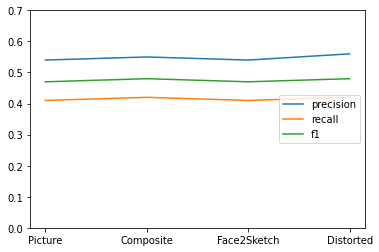
\includegraphics[width=50mm]{knn_micro}}}
  %\qquad
%\qquad
\subfloat[knn, macro]{
   % {\raisebox{1ex}% select appropriate amount
            { \frame{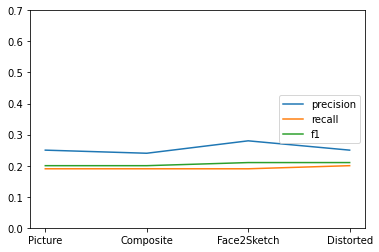
\includegraphics[width=50mm]{knn_macro}}}%
            %\frame{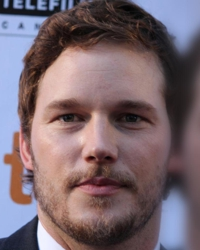
\includegraphics[width=40mm]{9737}}
            }
          %  }
\qquad
\subfloat[random forest, micro]{
   % {\raisebox{1ex}% select appropriate amount
            { \frame{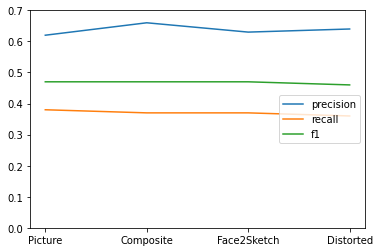
\includegraphics[width=50mm]{random_forest_micro}}}%
            %\frame{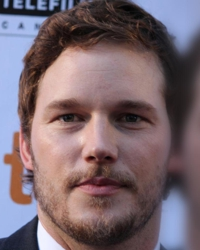
\includegraphics[width=40mm]{9737}}
            }
        %    }
%\qquad
\subfloat[random forest, macro]{
  %  {\raisebox{1ex}% select appropriate amount
            { \frame{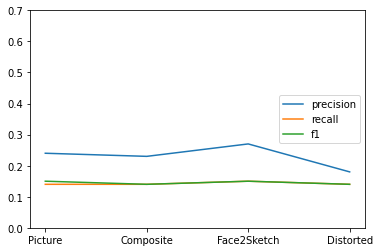
\includegraphics[width=50mm]{random_forest_macro}}}%
            %\frame{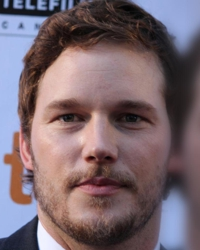
\includegraphics[width=40mm]{9737}}
            }
    %        }
%\qquad

\label{fig:taskdiff}
\end{figure}
\bigskip
\end{frame}


\begin{frame}
\frametitle{Conclusions and future work}
\begin{itemize}

\item In this study we examined the effects of visual and linguistic data augmentation
% as means of improving automatic generation of descriptions of human faces
\item Our results indicate that original images are generally more useful. However, it is still possible to ``distill'' original images to such level of abstractions (e.g., sketches), in which the model would still perform relatively well
\item The model benefits from training on captioning data from a different domain.
%Possibly, because from captions it learns general syntactic structures and a broader range of semantic relations between words. Descriptions of faces in the dataset are much more rigid in this respect.
\pause
\item Future work should focus on
\begin{itemize}
	\item improving the dataset to include more races, genders and ethnicities
	\item examining the possibility of representing images in terms of hierarchy of abstractions
	\item extending the task including descriptions in different languages
\end{itemize}

\pause
\textbf{Thank you for your attention!}

\end{itemize}
\end{frame}




\end{document}


%%% Local Variables:
%%% mode: latex
%%% mode: flyspell
%%% TeX-master: t
%%% TeX-PDF-mode: t
%%% coding: utf-8
%%% ispell-local-dictionary: "british"
%%% End:
